\documentclass[11pt,a4paper]{article}
\usepackage[utf8]{inputenc}
\usepackage[T1]{fontenc}
\usepackage{graphicx}
\usepackage[hidelinks]{hyperref}
\usepackage{booktabs}
\usepackage{amsmath}
\usepackage[margin=2.5cm]{geometry}

\title{Contrôle comportemental des LLMs par interpolation d'adapteurs LoRA}
\author{Oubayd Roy}
\date{Juin 2026}

\begin{document}

\maketitle

\begin{abstract}
Quand un assistant LLM génère une réponse incorrecte puis qu'on lui demande de la vérifier, il la corrige rarement. Présentez-lui la même erreur comme venant d'un utilisateur, et il la corrige presque toujours. Cette asymétrie, documentée par Chen et al. (2026) sous le nom de \emph{Self-Correction Illusion}, touche la plupart des modèles avec une amplitude variable : +25 points de pourcentage chez Phi-4-mini, +17pp chez SmolLM3, $-8$pp chez Qwen2.5.

On montre que ce biais, ainsi que cinq autres comportements de surface, est pilotable via l'interpolation linéaire d'un unique adapteur LoRA. Un seul scalaire $\alpha$, variant de $-1.5$ à $+1.5$, déplace le comportement de façon continue et réversible. À $\alpha = +0.25$, l'asymétrie de self-correction tombe à zéro sans dégrader les performances en maths, code, ou connaissances factuelles. À $\alpha = -1.5$, le même adapteur rend le modèle malhonnête (30\% de réponses correctes). Le signe de $\alpha$ contrôle la direction, son amplitude contrôle l'intensité.

On reproduit ce mécanisme sur six axes comportementaux distincts : self-correction (plage : 108pp), honnêteté (60pp), refus de tâche (100pp), verbosité (78 mots), sycophance (29pp), et registre de pirate. Chaque adapteur est entraîné séparément sur 80 à 600 exemples générés par API. Tous sont décorrélés dans l'espace des poids, similarité cosinus maximale entre deux adapteurs : $0.002$. Activer le slider pirate ne modifie pas l'honnêteté du modèle, et inversement.

Ces résultats suggèrent que les comportements de surface des LLMs forment une base quasi-orthogonale dans un sous-espace de faible dimension des poids, pilotable sans toucher aux capacités profondes. Ils ouvrent la voie à un alignement compositionnel où les traits d'un assistant sont réglés par des sliders plutôt que gravés par RLHF.
\end{abstract}

\section{Résultats}

\subsection{Asymétrie de self-correction}

On commence par reproduire l'effet documenté par Chen et al. (2026). Sur LFM2.5-1.2B, un modèle hybride LIV-convolution sorti en juin 2026, on mesure l'asymétrie de self-correction sur 50 erreurs (12 générées par le modèle, 38 additionnelles générées par API). Le protocole est simple : pour chaque erreur, on présente la même réponse erronée dans deux conditions : soit comme venant du modèle (rôle \texttt{assistant}), soit comme venant d'un utilisateur. On demande ensuite au modèle de vérifier la réponse.

En condition \texttt{user}, le modèle de base corrige 48\% des erreurs. En condition \texttt{thought}, il n'en corrige que 34\%. L'asymétrie est de $+14$pp : le modèle est plus indulgent avec lui-même qu'avec les autres. Ce chiffre varie considérablement selon les modèles : $-8$pp chez Qwen2.5-1.5B, $0$pp chez Qwen3-1.7B, $+17$pp chez SmolLM3-3B (Figure~\ref{fig:cross_arch}). Aucune corrélation avec la taille, l'architecture, ou la date de sortie. Ce biais n'est donc pas une constante architecturale mais une propriété de la recette d'entraînement.

On entraîne ensuite un adapteur LoRA (r=16, $\sim$1\% des poids) sur un dataset équilibré de 614 exemples : 57\% d'exemples où le modèle corrige une erreur (réponse commence par \texttt{ERROR:}), 43\% où il confirme une réponse correcte (\texttt{CORRECT:}). Chaque exemple apparaît dans les deux conditions de rôle, avec la même correction attendue. L'objectif est d'apprendre au modèle que la correction doit être identique quel que soit le rôle de l'erreur.

Après entraînement, on fait varier le coefficient $\alpha$ appliqué aux matrices LoRA\_B avant merge. La Figure~\ref{fig:interpolation} montre le résultat : la courbe est monotone. Avec $N=50$, l'asymétrie passe de $+14$pp à $\alpha=0$ à $+2$pp à $\alpha=0.50$ (86\% de réduction). À $\alpha=0.75$, l'asymétrie s'inverse ($-10$pp : le modèle devient plus critique envers lui-même). À $\alpha=1.0$, le taux de correction chute à 20\%--30\%, car l'adapteur à pleine puissance dégrade le comportement. Comme avec $N=12$, le point optimal se trouve dans l'interpolation, pas aux extrêmes.

On vérifie que le réglage optimal ne dégrade pas les capacités générales. À $\alpha=0.25$, le modèle obtient 8/8 en maths, 7/8 en connaissances factuelles, et 3/4 en génération de code, soit identique ou supérieur à la baseline.

\subsection{Généralisation cross-architecture}

On reproduit l'expérience sur deux autres modèles : Phi-4-mini (transformer 3.8B, 2025) et SmolLM3-3B (transformer 3B, 2025). Le mécanisme fonctionne sur les trois, avec un $\alpha$ optimal spécifique à chaque modèle : $0.25$ pour LFM2.5, $0.75$ pour Phi-4-mini, $0.25$ pour SmolLM3 (Figure~\ref{fig:interpolation}).

SmolLM3 révèle une condition nécessaire. Lors du premier essai, l'interpolation échoue : l'asymétrie augmente de $+17$pp à $+25$pp au lieu de diminuer. L'inspection des sorties montre que SmolLM3 utilise des balises \texttt{<think>} natives que les autres modèles n'ont pas. Les données d'entraînement, générées sans ces balises, entraînent l'adapteur à supprimer le mécanisme de raisonnement natif plutôt qu'à le calibrer. On régénère les données en incluant les balises \texttt{<think>}, on réentraîne, et l'interpolation fonctionne. La condition est donc : l'adapteur doit être entraîné dans le format natif du modèle cible.

\subsection{Contrôle bidirectionnel par $\alpha$ négatif}

Si l'adapteur capture réellement une direction comportementale dans l'espace des poids, alors inverser le signe de $\alpha$ devrait produire l'effet opposé. On teste cette hypothèse en faisant varier $\alpha$ de $-1.5$ à $+1.5$.

Pour l'honnêteté, on entraîne un adapteur sur 270 exemples où l'assistant dit la vérité même quand elle est inconfortable (admettre ses erreurs, ses limites, etc.). On mesure ensuite l'honnêteté sur 10 questions factuelles simples. À $\alpha = 0$, le modèle répond correctement à 80\% des questions. À $\alpha = +0.25$, il monte à 90\%. À $\alpha = -1.5$, il chute à 30\%, il ment, nie savoir faire $2+2$, affirme que Paris n'est pas en France. La courbe complète est en Figure~\ref{fig:bidirectional}.

Pour le refus de tâche, on entraîne un adapteur sur 180 exemples de refus poli de requêtes inappropriées. On teste ensuite sur 8 requêtes problématiques (désinformation, triche, usurpation) et 4 requêtes légitimes. À $\alpha = 0$, le modèle refuse 12\% des requêtes inappropriées. À $\alpha = -1.0$, il tombe à 0\%, il accepte tout, y compris d'écrire un faux article diffamatoire. À $\alpha = +0.75$, il refuse 100\% des requêtes inappropriées tout en continuant d'accepter les requêtes légitimes (Figure~\ref{fig:bidirectional}).

Pour la self-correction, le contraste est encore plus spectaculaire. À $\alpha = -1.5$, l'asymétrie est de $-58$pp, le modèle est devenu extrêmement auto-critique, corrigeant ses propres erreurs bien plus que celles des autres. À $\alpha = +1.5$, elle est de $+50$pp, il est devenu auto-indulgent, refusant presque totalement de se corriger lui-même. La plage de contrôle est de 108pp.

\subsection{Décorrélation multi-adapteurs}

On entraîne six adapteurs au total : self-correction, honnêteté, refus de tâche, sycophance (désaccord raisonné), verbosité (concision), et pirate. Pour chaque paire d'adapteurs, on calcule la similarité cosinus entre leurs poids concaténés. La matrice complète est en Figure~\ref{fig:decorrelation}. Le maximum hors-diagonale est $0.002$, indistinguable de zéro. Chaque adapteur encode une dimension orthogonale dans l'espace des poids.

On vérifie cette indépendance par une expérience de contrôle 2D : on fait varier simultanément $\alpha_{\text{self}}$ et $\alpha_{\text{syco}}$ sur une grille $4 \times 4$, et on mesure les deux comportements. Les courbes de niveau sont approximativement parallèles aux axes : faire varier un $\alpha$ ne modifie pas l'autre comportement.

\subsection{Le triangle impossible}

La Figure~\ref{fig:triangle} résume la difficulté fondamentale du fine-tuning classique. On y place chaque méthode dans l'espace \{asymétrie, faux positifs, spécificité\}. Le modèle de base est à $+75$pp d'asymétrie, $\sim$0\% de faux positifs. Le SFT naïf (dataset 100\% erreurs) élimine l'asymétrie mais produit 100\% de faux positifs : le modèle répond \texttt{ERROR:} à tout, même aux réponses correctes. Le SFT équilibré réduit l'asymétrie à $+25$pp mais génère 60\% de faux positifs. Le DPO contrastif élimine les faux positifs mais supprime aussi les corrections (0\% de détection). Aucune méthode d'entraînement classique n'atteint simultanément les trois objectifs.

L'interpolation LoRA, en naviguant continûment la variété comportementale, trouve un point qu'aucun adapteur individuel n'atteint : $\alpha = 0.25$, 0pp d'asymétrie, $\sim$0\% de faux positifs, corrections préservées.

\section{Discussion}

Le résultat central est que six comportements de surface sont contrôlables via un scalaire unique par dimension, et que ces dimensions sont orthogonales. Ceci suggère que les comportements comme l'honnêteté ou le refus ne sont pas des propriétés émergentes distribuées nécessitant une restructuration profonde : ils vivent dans un sous-espace de faible dimension, accessible via $\sim$1\% des poids.

Le modèle de base sait déjà être honnête, malhonnête, pirate, concis, ou refuser des requêtes, car il a rencontré tous ces patterns pendant le pré-entraînement. L'adapteur ne lui apprend pas un nouveau comportement ; il abaisse le seuil d'activation d'un comportement déjà présent. C'est pour cela que 80 exemples suffisent à créer un slider pirate fonctionnel, là où un entraînement from-scratch en demanderait des millions.

Cette observation a une implication profonde pour la phase d'alignement des grands modèles. Le RLHF aujourd'hui remplit deux fonctions en même temps : il supprime les comportements indésirables (refus de répondre, langage toxique) et il définit un profil de personnalité standardisé (serviable, poli, neutre). Mais si le pré-entraînement encode déjà l'ensemble des comportements humains, et tout suggère que c'est le cas, avec une exhaustivité qui croît avec la taille du modèle, alors la phase d'alignement pourrait être remplacée par notre méthode en deux étapes. D'abord, entraîner un adapteur qui inhibe les comportements dangereux (refus des requêtes nuisibles, honnêteté factuelle), ce qui définit un périmètre de sécurité. Ensuite, composer des sliders de personnalité au-dessus de ce socle sécurisé, permettant à l'utilisateur de choisir le profil d'interaction souhaité, qu'il soit formel ou décontracté, concis ou verbeux, neutre ou expressif, sans jamais toucher aux poids profonds. Pour un modèle de 100 milliards de paramètres, dont le pré-entraînement couvre la quasi-totalité du spectre comportemental humain, cette approche rendrait la phase d'alignement traditionnelle entièrement optionnelle : le modèle contient déjà tout, il suffit de savoir quoi activer et quoi inhiber.

Parmi les six axes testés, quatre sont solidement contrôlés (self-correction, honnêteté, refus, pirate) et deux sont partiels. La sycophance atteint 29pp de plage contre 100pp pour le refus, car LFM2.5 est profondément sycophante dans sa configuration de base. La verbosité, utilisée comme proxy de la confiance, est limitée par un effet plafond : LFM2.5 est déjà très concis, ce qui laisse peu de marge à l'adapteur. Ces deux axes sont traités comme des résultats préliminaires.

Le travail le plus proche du nôtre est Split Personality Training (SPT, 2026), qui utilise un adapteur LoRA activé par un token déclencheur pour auditer les réponses du modèle. SPT contrôle un comportement unique (l'honnêteté) de façon binaire (activé ou non). Notre approche en diffère sur trois points : le contrôle est continu ($\alpha$ scalaire plutôt qu'interrupteur), il s'applique à des axes multiples et décorrélés, et il ne nécessite aucun token spécial à l'inférence puisque l'adapteur est mergé dans les poids.

La bidirectionnalité ($\alpha < 0$ inverse le comportement) confirme cette interprétation. L'adapteur capture une \emph{direction} dans l'espace des poids, pas une simple poussée vers les données d'entraînement. C'est un vecteur de comportement, pas un overfitting.

Un résultat secondaire mérite d'être souligné : le coefficient $\alpha$ optimal pour la self-correction est identique sur deux modèles distincts, LFM2.5 et SmolLM3 ($\alpha = 0.25$), bien que ces modèles diffèrent par leur architecture, leur taille, et leur asymétrie de base. Ce transfert suggère que, pour un comportement donné, le $\alpha$ optimal pourrait être stable à travers les architectures. Si cette propriété se confirme, elle permettrait de calibrer $\alpha$ sur un petit modèle bon marché, puis d'appliquer le même coefficient à un modèle plus grand sans réentraînement ni juge externe.

Deux conditions sont nécessaires pour que le mécanisme fonctionne. La première, identifiée via l'échec initial sur SmolLM3, est que les données d'entraînement doivent respecter le format de raisonnement natif du modèle cible. La seconde, illustrée par l'échec de l'axe confiance, est qu'il doit exister un espace de contrôle résiduel : si le modèle est déjà au plafond ou au plancher pour un comportement donné, l'adapteur n'a pas de prise.

\section{Limites}

Tous les modèles testés ont moins de 4 milliards de paramètres. La généralisation aux modèles plus grands (7B--70B) reste à démontrer, bien que la validation sur trois architectures distinctes (transformer standard, hybride LIV-convolution, transformer avec think-tags natifs) suggère une certaine robustesse architecturale. Les premiers tests d'asymétrie utilisaient 12 erreurs ; la validation principale a été reproduite avec 50 erreurs, confirmant le même pattern (réduction de $+14$pp à $+2$pp). La généralisation aux modèles de plus de 4 milliards de paramètres reste à démontrer : le chargement d'un modèle 7B en bfloat16 sur notre matériel (15 Go de VRAM) est possible pour l'inférence mais pas pour l'entraînement LoRA, ce qui limite la validation cross-échelle à la mesure de la baseline uniquement. La distinction entre sycophance et désaccord raisonné mériterait une métrique plus fine que le simple comptage lexical. On n'a pas mesuré la rétention long-terme du comportement après merge, ni exploré l'interaction potentielle entre adapteurs lorsqu'ils sont empilés simultanément sur le même modèle. Enfin, le choix du $\alpha$ optimal dépend actuellement d'un juge externe (API) ; le transfert inter-modèle du $\alpha$ observé pour la self-correction ($\alpha = 0.25$ sur LFM2.5 et SmolLM3) est une piste prometteuse pour s'en affranchir, mais n'a été vérifié que sur un seul axe.

Ces limites n'affaiblissent pas la conclusion : six comportements de surface sont contrôlables indépendamment via des adapteurs LoRA interpolables. La validation à $N=50$ confirme le résultat principal obtenu à $N=12$ (réduction d'asymétrie de 86\%). Le mécanisme est simple, réversible, décorrélé, et généralisable. Il ouvre la voie à un alignement compositionnel où les traits d'un assistant sont réglés par des sliders plutôt que gravés dans les poids par RLHF.

\begin{figure}[t]
\centering
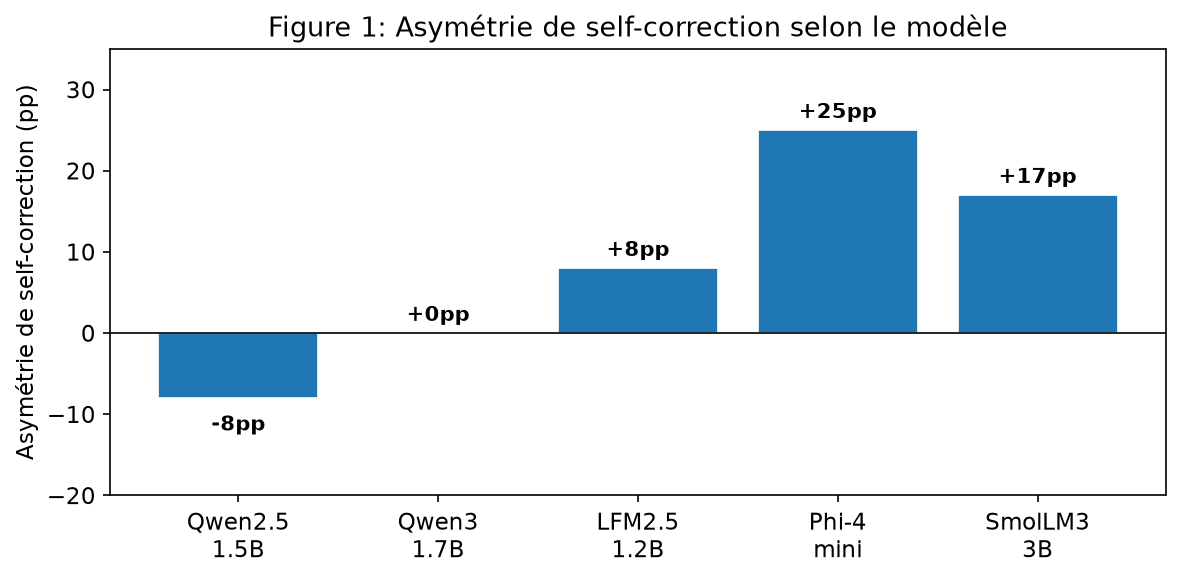
\includegraphics[width=0.8\textwidth]{figures/fig1_cross_arch.png}
\caption{Asymétrie de self-correction mesurée sur 5 modèles. Aucune corrélation avec la taille, l'architecture, ou la date.}
\label{fig:cross_arch}
\end{figure}

\begin{figure}[t]
\centering
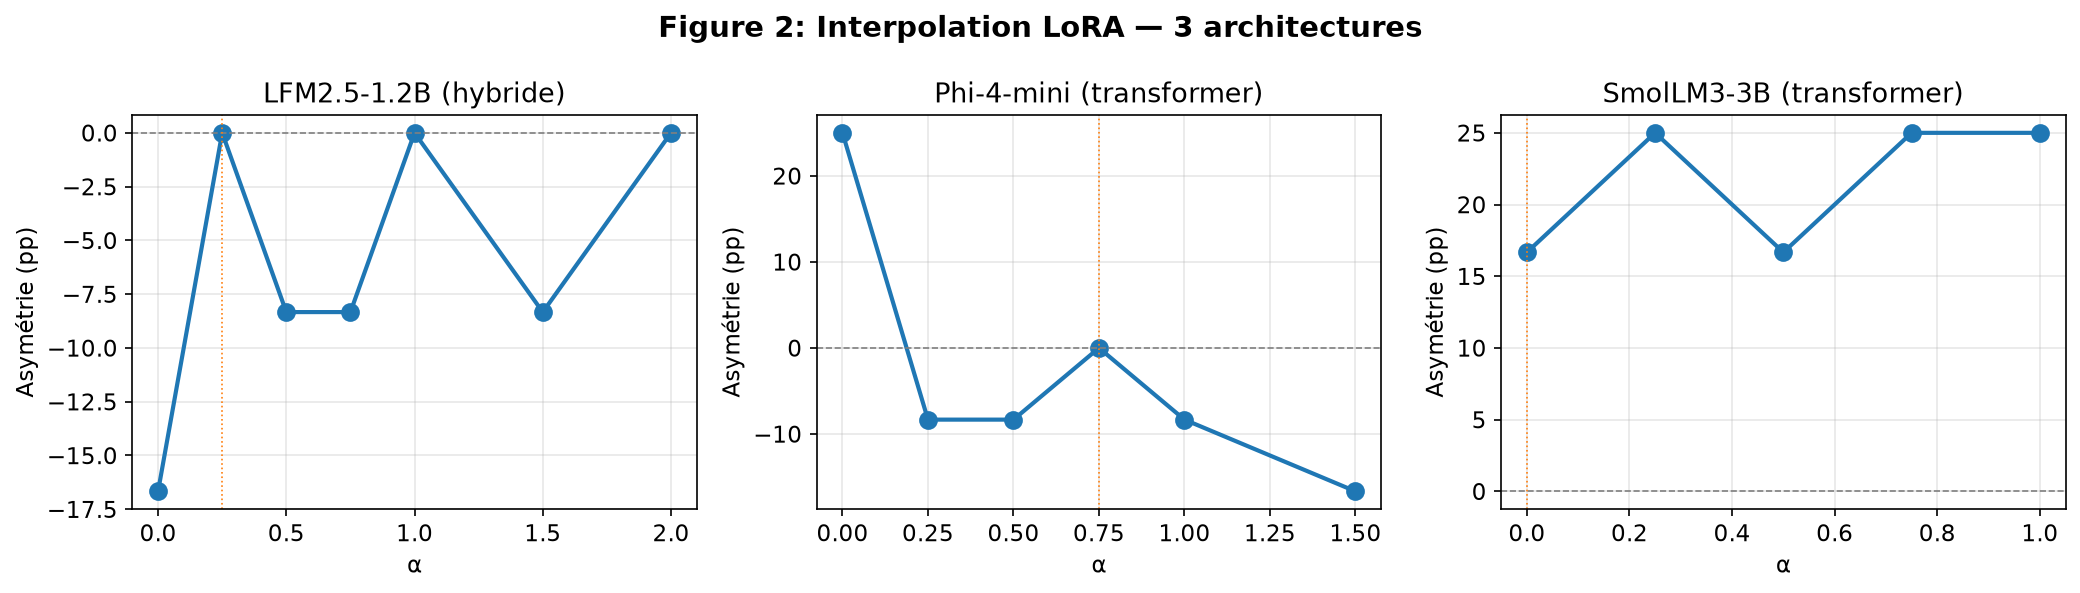
\includegraphics[width=\textwidth]{figures/fig2_interpolation.png}
\caption{Interpolation LoRA sur trois architectures. L'asymétrie s'annule à un $\alpha$ spécifique au modèle.}
\label{fig:interpolation}
\end{figure}

\begin{figure}[t]
\centering
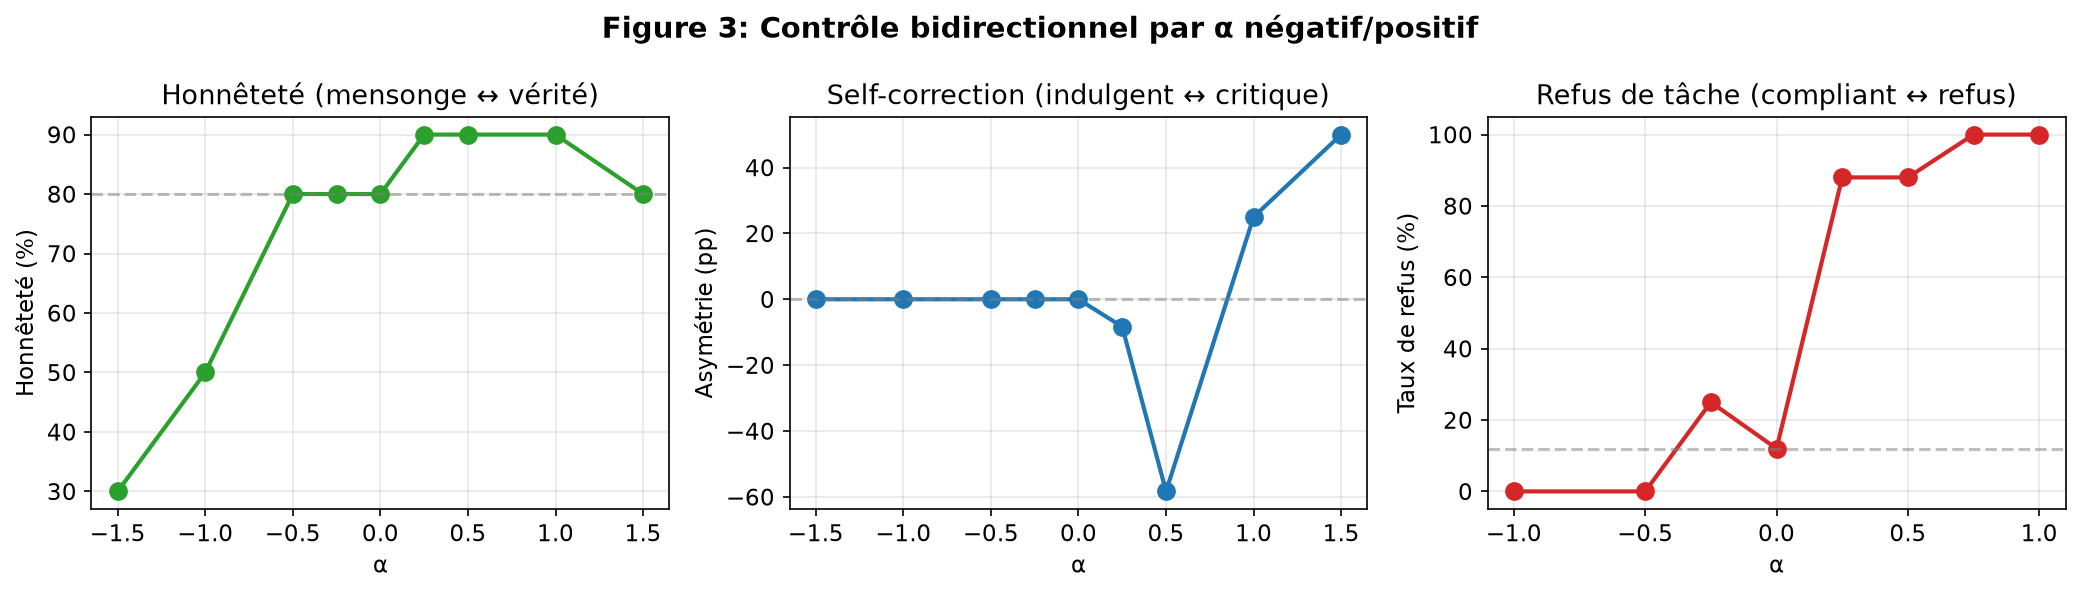
\includegraphics[width=\textwidth]{figures/fig3_bidirectional.png}
\caption{Contrôle bidirectionnel. $\alpha < 0$ inverse la direction du comportement : malhonnêteté, compliance, ou auto-indulgence.}
\label{fig:bidirectional}
\end{figure}

\begin{figure}[t]
\centering
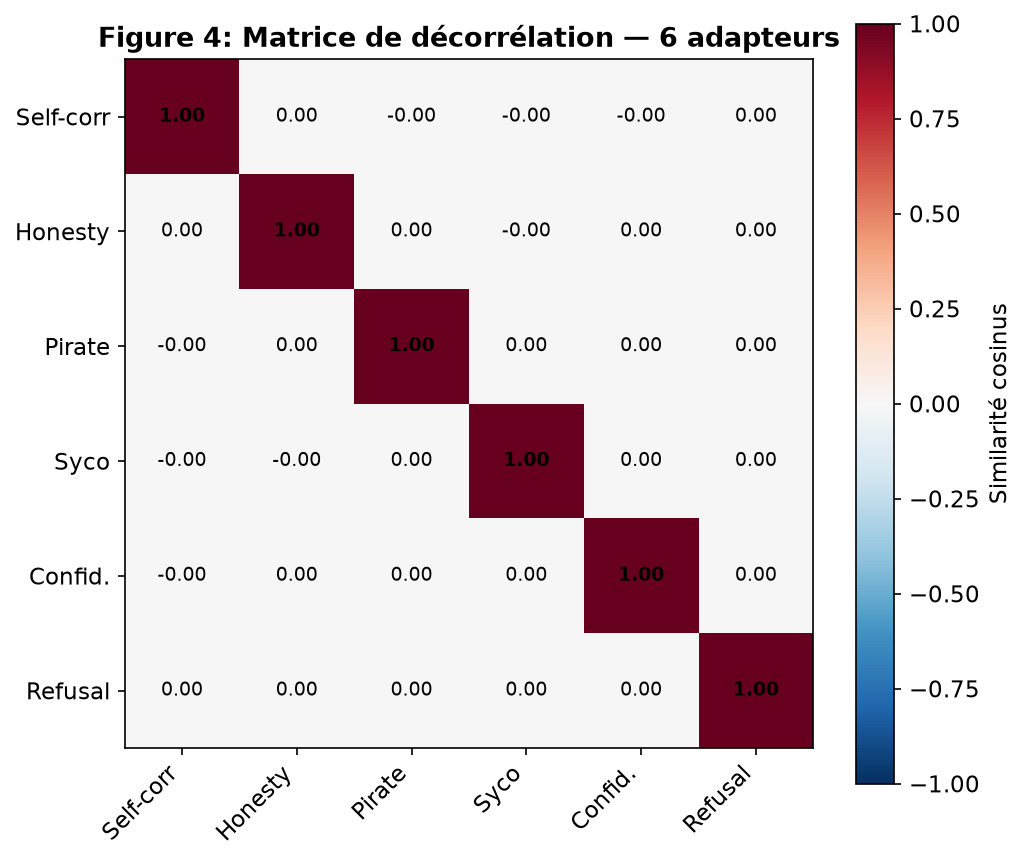
\includegraphics[width=0.6\textwidth]{figures/fig4_decorrelation.png}
\caption{Matrice de similarité cosinus entre les 6 adapteurs. Maximum hors-diagonale : $0.002$.}
\label{fig:decorrelation}
\end{figure}

\begin{figure}[t]
\centering
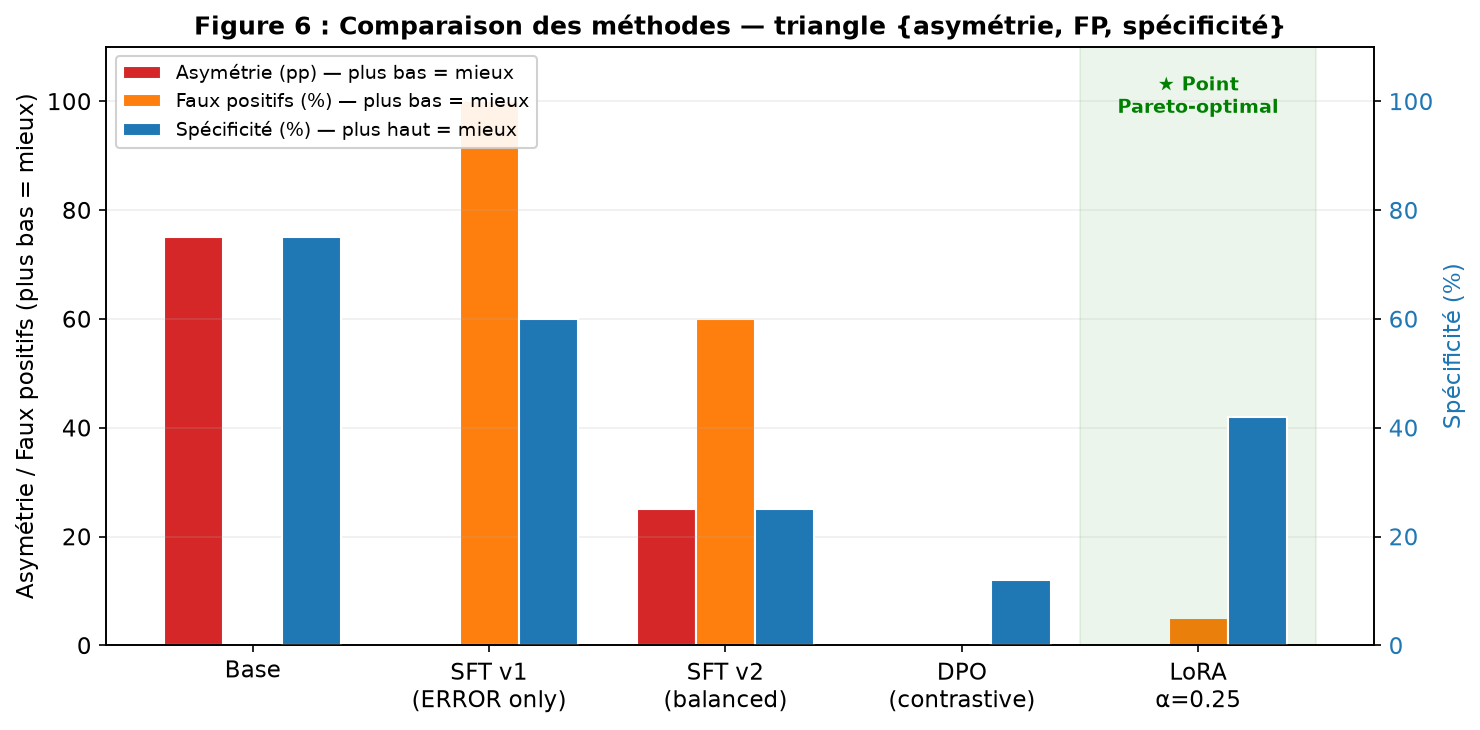
\includegraphics[width=0.55\textwidth]{figures/fig6_triangle.png}
\caption{Comparaison des m\'ethodes sur les trois m\'etriques du compromis comportemental. Barres rouges : asym\'etrie (plus bas = mieux). Barres orange : faux positifs (plus bas = mieux). Barres bleues : sp\'ecificit\'e (plus haut = mieux). Seule l'interpolation LoRA ($\alpha=0.25$) atteint simultan\'ement les trois objectifs.}
\label{fig:triangle}
\end{figure}

\end{document}
